\documentclass{beamer}

% Beamer style
%\usetheme[secheader]{Madrid}
\usetheme{CambridgeUS}
\usecolortheme[rgb={0.65,0.15,0.25}]{structure}
%\usefonttheme[onlymath]{serif}
\beamertemplatenavigationsymbolsempty
%\AtBeginSubsection

% Packages
%\usepackage[french]{babel}
\usepackage[latin1]{inputenc}
%\usepackage[utf8]{inputenc}
\usepackage{color}
\usepackage{dsfont, stmaryrd}
\usepackage{amsmath, amsfonts, amssymb}
\usepackage{stmaryrd}
\usepackage{epsfig}
\usepackage{url}
\usepackage{/media/donnees/LATEX/astats}
%\usepackage[all]{xy}
\usepackage{graphicx}

% Commands
\definecolor{darkred}{rgb}{0.65,0.15,0.25}
\newcommand{\emphase}[1]{\textcolor{darkred}{#1}}
\newcommand{\paragraph}[1]{\emphase{#1}}
\newcommand{\refer}[1]{\textcolor{blue}{\sl \cite{#1}}}
\newcommand{\Refer}[1]{\textcolor{blue}{\sl #1}}
\newcommand{\newblock}{}

% Symbols
\newcommand{\Abf}{{\bf A}}
\newcommand{\Acal}{\mathcal{A}}
\newcommand{\Beta}{\text{B}}
%\newcommand{\betabf}{\mbox{\mathversion{bold}{$\beta$}}}
\newcommand{\Bcal}{\mathcal{B}}
\newcommand{\BIC}{\text{BIC}}
\newcommand{\dd}{\text{d}}
\newcommand{\dbf}{{\bf d}}
\newcommand{\Dcal}{\mathcal{D}}
\newcommand{\Esp}{\mathbb{E}}
\newcommand{\Ebf}{{\bf E}}
\newcommand{\Ecal}{\mathcal{E}}
\newcommand{\Gcal}{\mathcal{G}}
\newcommand{\Gam}{\mathcal{G}\mbox{am}}
\newcommand{\Ibb}{\mathbb{I}}
\newcommand{\Ibf}{{\bf I}}
\newcommand{\ICL}{\text{ICL}}
\newcommand{\Cov}{\mathbb{C}\text{ov}}
\newcommand{\Corr}{\mathbb{C}\text{orr}}
\newcommand{\Var}{\mathbb{V}}
\newcommand{\Vsf}{\mathsf{V}}
\newcommand{\pen}{\text{pen}}
\newcommand{\Fcal}{\mathcal{F}}
\newcommand{\Hbf}{{\bf H}}
\newcommand{\Hcal}{\mathcal{H}}
\newcommand{\Jcal}{\mathcal{J}}
\newcommand{\Kbf}{{\bf K}}
\newcommand{\Lcal}{\mathcal{L}}
\newcommand{\Mcal}{\mathcal{M}}
\newcommand{\mbf}{{\bf m}}
\newcommand{\mum}{\mu(\mbf)}
\newcommand{\Ncal}{\mathcal{N}}
\newcommand{\Nbf}{{\bf N}}
\newcommand{\Nm}{N(\mbf)}
\newcommand{\Ocal}{\mathcal{O}}
\newcommand{\Obf}{{\bf 0}}
\newcommand{\Omegas}{\underset{s}{\Omega}}
\newcommand{\Pbf}{{\bf P}}
\newcommand{\Pcal}{\mathcal{P}}
\newcommand{\Qcal}{\mathcal{Q}}
\newcommand{\Rbb}{\mathbb{R}}
\newcommand{\Rcal}{\mathcal{R}}
\newcommand{\sbf}{{\bf s}}
\newcommand{\Sbf}{{\bf S}}
\newcommand{\Scal}{\mathcal{S}}
\newcommand{\Ucal}{\mathcal{U}}
\newcommand{\Vcal}{\mathcal{V}}
\newcommand{\Tbf}{{\bf T}}
\newcommand{\ubf}{{\bf u}}
\newcommand{\Ubf}{{\bf U}}
\newcommand{\Wbf}{{\bf W}}
\newcommand{\xbf}{{\bf x}}
\newcommand{\Xbf}{{\bf X}}
\newcommand{\ybf}{{\bf y}}
\newcommand{\Ybf}{{\bf Y}}
\newcommand{\Zbf}{{\bf Z}}
\newcommand{\pibf}{\mbox{\mathversion{bold}{$\pi$}}}
\newcommand{\Sigmabf}{\mbox{\mathversion{bold}{$\Sigma$}}}
\newcommand{\gammabf}{\mbox{\mathversion{bold}{$\gamma$}}}
\newcommand{\mubf}{\mbox{\mathversion{bold}{$\mu$}}}
\newcommand{\nubf}{\mbox{\mathversion{bold}{$\nu$}}}
%\newcommand{\Thetabf}{\mbox{\mathversion{bold}{$\Theta$}}}
\newcommand{\thetabf}{\mbox{\mathversion{bold}{$\theta$}}}
\newcommand{\BP}{\text{BP}}
\newcommand{\EM}{\text{EM}}
\newcommand{\VEM}{\text{VEM}}
\newcommand{\VBEM}{\text{VB}}
\newcommand{\cst}{\text{cst}}
\newcommand{\obs}{\text{obs}}
\newcommand{\ra}{\emphase{$\rightarrow$~}}
\newcommand{\QZ}{Q_{\Zbf}}
\newcommand{\Qt}{Q_{\thetabf}}

\newcommand{\Pause}{\pause}

% Directory
\newcommand{\fignet}{/media/donnees/RECHERCHE/RESEAUX/EXPOSES/FIGURES}
\newcommand{\figmotif}{/media/donnees/RECHERCHE/RESEAUX/MOTIFS/FIGURES}
\newcommand{\figgenet}{/media/donnees/RECHERCHE/GENETIQUE/EXPOSE/Figures}

%====================================================================
%====================================================================
% Some statistical aspects of biological network analysis

% Stéphane Robin

% UMR 518 AgroParisTech / INRA Applied Mathematics and Computer Sciences

% Network analysis has become a major challenge in biology as network is
% a natural way to describe interactions between molecules, individual,
% species, etc. Networks are also interesting from a statistical point
% of view as they constitute a very specific data structure. In the last
% decade, many statistical developments have been inspired by biological
% network analysis. The aim of this talk is to introduce some of them,
% focusing on several works recently developed within the ANR program
% 'Network Motif'.

% Understanding gene regulation is a key issue to better understand the
% functioning of the cell as a whole. Many efforts have been put on the
% inference of the regulatory network, based on expression data. The
% Gaussian graphical model (GGM) rapidly emerged as an efficient
% framework, where the inference of the network can be related to these
% of an (inverse) covariance matrix. As the network is expected to be
% sparse, regularized (or penalized) regression techniques are often
% used. The form of the regularization term can be adapted to account
% for some prior information about the network to be inferred.

% Many data are now represented as graphs of large size. In such
% networks, the nodes most often display very heterogeneous connectivity
% profiles, making most naive random graph models irrelevant. Mixture
% models are a classical way in statistics to retrieve some underlying
% structure among objects. The stochastic-block model (SBM) is a mixture
% model for random graph, and some progresses have been recently made
% about its inference. As it is an explicit statistical model, the SBM
% can be enriched to account for exogenous information.

% The structure of a network can also be studied at a lower scale,
% trying to isolate recurrent local patterns that could be interpreted
% as building blocks of the network. Most informative patterns (also
% call 'motifs') are expected to be either over- or under-represented,
% with respect to some relevant null model. The detection of exceptional
% motifs in a graph raises interesting issues both in algorithmics and
% in statistics.

%====================================================================
%====================================================================
\title[Some Statistics for Biological Networks]{Some Statistical
  Aspects of Biological Networks Analysis: The NeMo project}

\author{S. Robin}

\institute[AgroParisTech/INRA]{AgroParisTech / INRA \\
  \bigskip
  \begin{tabular}{ccccc}
    
\epsfig{file=\fignet/LogoINRA-Couleur.ps, width=2.5cm} & 
    \hspace{.5cm} &
    
\epsfig{file=\fignet/logagroptechsolo.eps, width=3.75cm} & 
    \hspace{.5cm} &
    
\epsfig{file=\fignet/logo-ssb.eps, width=2.5cm} \\ 
  \end{tabular} \\
  \bigskip
}

\date[GdR BIM 2012, Paris]{Journées du GdR Bio-Informatique
  Moléculaire, January 2012, Paris}

%====================================================================

%====================================================================
%====================================================================
\begin{document}
%====================================================================
%====================================================================

%====================================================================
\frame{\titlepage}
%====================================================================

% Because the living of a cell is basically governed by the interactions
% between its components, biological network have become a central
% object is the recent years. The third lecture will introduce different
% kind of network and discuss some statistical aspects regarding their
% inference, their evolution, their dynamics or the analysis of their
% topological properties.

%====================================================================
\section{Biological Networks}
%\frame{ \frametitle{Biological Networks} }
%====================================================================

%====================================================================
\subsection{The NeMo Project}
\frame{ \frametitle{The NeMo Project} 
%====================================================================
  \begin{tabular}{cc}
    \hspace{-.5cm}
    \begin{tabular}{p{.5\textwidth}}
      \paragraph{Call:} ANR Blanc 2008 \\
      Mathématique et Interactions.  \Pause \\
      \\
      \paragraph{3 partners:}
      \begin{enumerate}
      \item UMR 518 AgroParisTech / INRA MIA, Paris + INRA-MIG, Jouy
      \item UMR 8071 Statistique et Génome, Evry
      \item BAOBAB Team, INRIA / LBBE, Lyon
      \end{enumerate} \Pause
    \end{tabular}
    & 
    \hspace{-.5cm}
    \begin{tabular}{p{.5\textwidth}}
      \paragraph{Research topic:}
      \begin{enumerate}
      \item Network inference
      \item Random graph models for biological networks
      \item Detection of exceptional network motifs
      \end{enumerate}  
      \\ \Pause
      \paragraph{and also}
      \begin{itemize}
      \item Network comparison
      \item Data integration
      \end{itemize}
    \end{tabular}
  \end{tabular}

  \paragraph{Website: \url{nemo.ssbgroup.fr/} }
}

%====================================================================
\section{Network Inference}
\frame{ \frametitle{Network Inference} }
%====================================================================

%====================================================================
\subsection{Gaussian graphical models}
\frame{ \frametitle{Gaussian graphical models}
%====================================================================

  \paragraph{A generic problem:} Infer gene regulation networks from
  gene expression data.
  
  \bigskip
  \paragraph{Main idea:} Correlations between gene expression profiles
  inform us about regulation mechanisms between genes.

  \bigskip\bigskip\Pause
  \paragraph{A standard (and convenient) model: Gaussian graphical
    model (GGM). } \\
  Denoting 
  $$
  Y_{ik} = \text{expression level of gene $i$ ($=1\dots p$) in replicate
    $k (=1\dots n)$},
  $$
  suppose that the replicates are all independent and Gaussian:
  $$
  \Ybf_k = (Y_{1k} \dots Y_{pk}), 
  \qquad
  \{\Ybf_k\} \text { i.i.d. } \Ncal(\mubf, \Sigmabf)
  $$
  \ra $\Sigmabf$ reveals correlations ('\emphase{co-expressions}').
  }

%====================================================================
\frame{ \frametitle{Gaussian graphical models}

  \begin{tabular}{cc}
    \hspace{-.5cm}
    \begin{tabular}{p{.45\textwidth}}
      \paragraph{Spurious edges.} \\ 
      % \begin{overprint}
      %   \onslide<2>
      %   \epsfig{file=../FIGURES/GGM-Corr-1.eps, clip=,
      %     width=1\textwidth}
      %   \onslide<3>
      %   \epsfig{file=../FIGURES/GGM-Corr-2.eps, clip=,
      %     width=1\textwidth}
      %   \onslide<4->
      \epsfig{file=../FIGURES/GGM-Corr-3.eps, clip=,
        width=.8\textwidth} \Pause
      % \end{overprint}
      
      \vspace{-4cm} The elements of $\Sigmabf$ (and
      $\widehat{\Sigmabf}$) are expected to be \emphase{mostly
        non-zero}, whereas the network is expected to be
      \emphase{sparse}. \Pause
    \end{tabular}
    & 
    \hspace{-.5cm}
    \begin{tabular}{p{.5\textwidth}}
      \paragraph{'Regulatory' network.} Only 'direct', i.e. conditional
      correlations matters: 
      $$
      p_{ij} = \rho(Y_i, Y_j | \Ybf^{\setminus ij})
      $$ \Pause
      
      \paragraph{Property of GGM:}
      $$
      p_{ij} = -w_{ij} \left/ \sqrt{w_{ii} w_{jj}} \right.
      $$
      where
      $$
      \Wbf = (w_{ij}) = \Sigmabf^{-1}
      $$
      Regulations are revealed by the \emphase{non-zero terms of the
        precision matrix $\Wbf$.} 
      \vspace{2cm}~ 
    \end{tabular}
  \end{tabular}
}

%====================================================================
\subsection{Inferring the precision matrix}
% \frame{ \frametitle{Inferring the precision matrix}
% %====================================================================
%   \begin{tabular}{cc}
%     \hspace{-.5cm}
%     \begin{tabular}{p{.4\textwidth}}
%       \paragraph{Major issue: $p \gg n$} \\
%       \ra $\widehat{\Sigmabf}$ is singular. \\
%       \ra $\widehat{\Sigmabf}^{-1}$ does not exist. \\ \Pause
      
%       \\~\\
%       \paragraph{Some strategies:}
%       \begin{itemize}
%       \item Multiple testing
%       \item (Penalized) regression
%       \item Regularization of $\widehat{\Wbf}$ \emphase{toward
%           sparsity}.
%       \end{itemize} \Pause
%       \\~\\
      
%       \paragraph{Result = Undirected graph} \\
%       (while regulation is oriented). \\
%     \end{tabular}

%     & 
%     \hspace{-.5cm}
%     \begin{tabular}{p{.5\textwidth}}
%       \epsfig{file = \fignet/ScS05-SAGMD-Fig5.ps, clip=, bbllx=110,
%       bblly=225, bburx=310, bbury=375, height=.7\textheight,
%       width=.5\textwidth} \\ 
%     (source Schäffer \& Strimmer, 05)
% %    (\refer{ScS05})
%   \end{tabular}
%   \end{tabular}
%   }

%==================================================================== 
\frame{ \frametitle{Regularization via penalization} 

  \begin{tabular}{cc}
    \hspace{-.45cm}
    \begin{tabular}{p{.45\textwidth}}
      \onslide+<1->{
        \paragraph{Major issue: $p \gg n$} \\
        \ra $\widehat{\Sigmabf}$ is singular. \\
        \ra $\widehat{\Wbf} = \widehat{\Sigmabf}^{-1}$ does not
        exist. \\ \Pause 
      }
      
      \onslide+<2->{
        \bigskip
        \paragraph{Regularized estimate of $\Wbf$.} \\
        Rather than regular maximum-likelihood
        $$
        \widehat{\Wbf} = \arg\max_{\Wbf} \Lcal(\Ybf; \Wbf)
        $$
        consider
        $$
        \max_{\Wbf} \Lcal(\Ybf; \Wbf) - \lambda \; \text{pen}(\Wbf)
        $$
        \vspace{2cm}~
      }
    \end{tabular}
    & 
    \hspace{-.75cm}
    \begin{tabular}{p{.55\textwidth}}
      \onslide+<3->{
        \paragraph{Regularization.}
        Geometric view. \\
      }
      
      \begin{overprint}
        \onslide<3> 
        \vspace{.92cm} 
        $~ \qquad \max_{\thetabf} \Lcal(\Ybf, \thetabf)$ \\~\\
        \epsfig{file=\figgenet/Reg-Theta.eps,
          clip=, width=0.7\textwidth} 
        % \onslide<4>
        % \emphase{Ridge penalty:}  \\~\\
        % $ ~\qquad \max_{\thetabf} \Lcal(\Ybf, \thetabf) +
        % \lambda \|\thetabf\|_2^2 $  \\~\\
        % \epsfig{file=\figgenet/Reg-Ridge1.eps, clip=,
        %   width=0.7\textwidth} 
        \onslide<4>
        \emphase{Ridge penalty:}  \\~\\
        $ ~\qquad \max_{\thetabf} \Lcal(\Ybf, \thetabf) +
        \lambda \|\thetabf\|_2^2
        $ \\~\\
        \epsfig{file=\figgenet/Reg-Ridge2.eps, clip=,
          width=0.7\textwidth} 
        % \onslide<6>
        % \emphase{LASSO penalty:} \\~\\
        % $ ~\qquad \max_{\thetabf} \Lcal(\Ybf, \thetabf) +
        % \lambda \|\thetabf\|_1
        % $ \\~\\
        % \epsfig{file=\figgenet/Reg-Lasso1.eps, clip=,
        %   width=0.7\textwidth} 
        \onslide<5>
        \emphase{LASSO penalty:} \\~\\
        $ ~\qquad \max_{\thetabf} \Lcal(\Ybf, \thetabf) +
        \lambda \|\thetabf\|_1
        $ \\~\\
        \epsfig{file=\figgenet/Reg-Lasso2.eps, clip=,
          width=0.7\textwidth}
      \end{overprint}
      
    \end{tabular}
  \end{tabular}

}

% %==================================================================== 
% \frame{ \frametitle{Penalization for the precision matrix} 

%   \paragraph{Penalized likelihood.} Denoting $\Ybf$ gene expression
%   data, we look for
%   $$
%   \widehat{\Wbf} = \arg\max_\Wbf \left[\Lcal(\Wbf; \Ybf) -
%     \text{pen}(\Wbf)\right] 
%   $$
%   where $\Lcal$ denote the log-likelihood: $\Lcal(\Wbf; \Ybf) = \log
%   P(\Ybf | \Wbf)$.

%   \bigskip\bigskip\Pause
%   \paragraph{$\ell_1$ penalization ensures sparsity}
% %  \refer{BEA08} propose to maximize
%   $$
%   \arg\max \Lcal(\Ybf; \Wbf) - \lambda \|\Wbf\|_1
%   \qquad \text{where} \qquad
%   \|\Wbf\|_1 = \sum_{i, j} w_{ij}.
%   $$

%   \bigskip\Pause
%   \emphase{A (more tractable) pseudo-likelihood} is sometimes
%   used:
%   $$
%   \widetilde{\Lcal}(\Wbf; \Ybf) = \log \prod_i P(\Ybf_i |
%   \Ybf^{\setminus i}, \Wbf).
%   $$
%   \refer{ACM09} showed that neighborhood selection 
%   % (\refer{MeB06})
%   corresponds to pseudo-likelihood $\ell_1$-penalization.  
% }

%==================================================================== 
\subsection{Playing with penalties}
\frame{ \frametitle{Playing with penalties: Multi-task learning} 
%==================================================================== 
    \paragraph{Several conditions.} Suppose we deal with $T$
    experimental conditions and observe $T$ gene expression datasets:
    $\Ybf_1, \dots, \Ybf_T$.
    
    \bigskip \Pause
    \paragraph{Independent networks.} One may fit the one network
    $\Wbf^t$ for each condition:
    $$
    \text{for } t = 1\dots T, \qquad \max_\Wbf \widetilde{\Lcal}(\Ybf^t;
    \Wbf^t) - \lambda \|\Wbf^t\|_1 
    %\qquad \text{where } \|\Wbf^t\|_1 = \sum_{i, j} |w_{ij}|
    \Pause
    $$
    \begin{tabular}{cc}
      \hspace{-.5cm}
      \begin{tabular}{p{.3\textwidth}}
        Or rather assume that \emphase{the $T$ networks $\Wbf^t$ share
          some similarities}.  \\
       ~\\
        \refer{CGA11}
      \end{tabular}
      & 
      \hspace{-.5cm}
      \begin{tabular}{p{.5\textwidth}}
        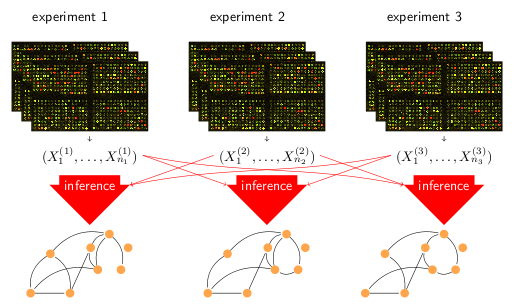
\epsfig{file=\fignet/multitask.eps, clip=, width=0.6\textwidth} 
      \end{tabular}
    \end{tabular}
  }

%==================================================================== 
\frame{ \frametitle{Playing with penalties: Multi-task learning} 
  \onslide+<1->{
    \paragraph{Sharing information.} \refer{CGA11} \\ 
  } 
  \begin{overprint}
    \onslide<1>
    Graphical group-LASSO:
    $$
    \max_{\Wbf^1, \dots, \Wbf^T} \sum_t \widetilde{\Lcal}(\Ybf^t;
    \Wbf^t) - \lambda \sum_{i \neq j} \sqrt{\sum_t
      \left(w_{ij}^t\right)^2}.
    $$
    \begin{tabular}{cc}
      \hspace{-.5cm}
      \begin{tabular}{p{.4\textwidth}}
        \begin{itemize}
        \item[\ra] all networks have the \emphase{same topology} (same
          0's in $\Wbf^t$).
        \end{itemize}
        \vspace{5cm}~ 
      \end{tabular}
      & 
      \hspace{-.5cm}
      \begin{tabular}{p{.6\textwidth}}
      \end{tabular}
    \end{tabular}
    \onslide<2->
    Graphical cooperative-LASSO: 
    $$
    \max_{\Wbf^1, \dots, \Wbf^T} \sum_t
    \widetilde{\Lcal}(\Ybf^t; \Wbf^t)- \lambda \sum_{i \neq j}
    \sqrt{\sum_t \left[w_{ij}^t\right]_{\emphase{+}}^2}+ \lambda
    \sum_{i \neq j} \sqrt{\sum_t
      \left[w_{ij}^t\right]_{\emphase{-}}^2}.
    $$
    \vspace{-0.5cm}
    \begin{tabular}{cc}
      \hspace{-.5cm}
      \begin{tabular}{p{.4\textwidth}}
        \begin{itemize}
        \item[\ra] networks have \emphase{similar topologies},
        \item[\ra] coefficients keep the \emphase{same sign} (same
          regulation direction).
        \end{itemize} \\
        
        \paragraph{2 conditions (ER+/ER-).} \\
        \refer{JCG12}
        \vspace{4cm}~ 
      \end{tabular}
      & 
      \hspace{-.5cm}
      \begin{tabular}{p{.6\textwidth}}
        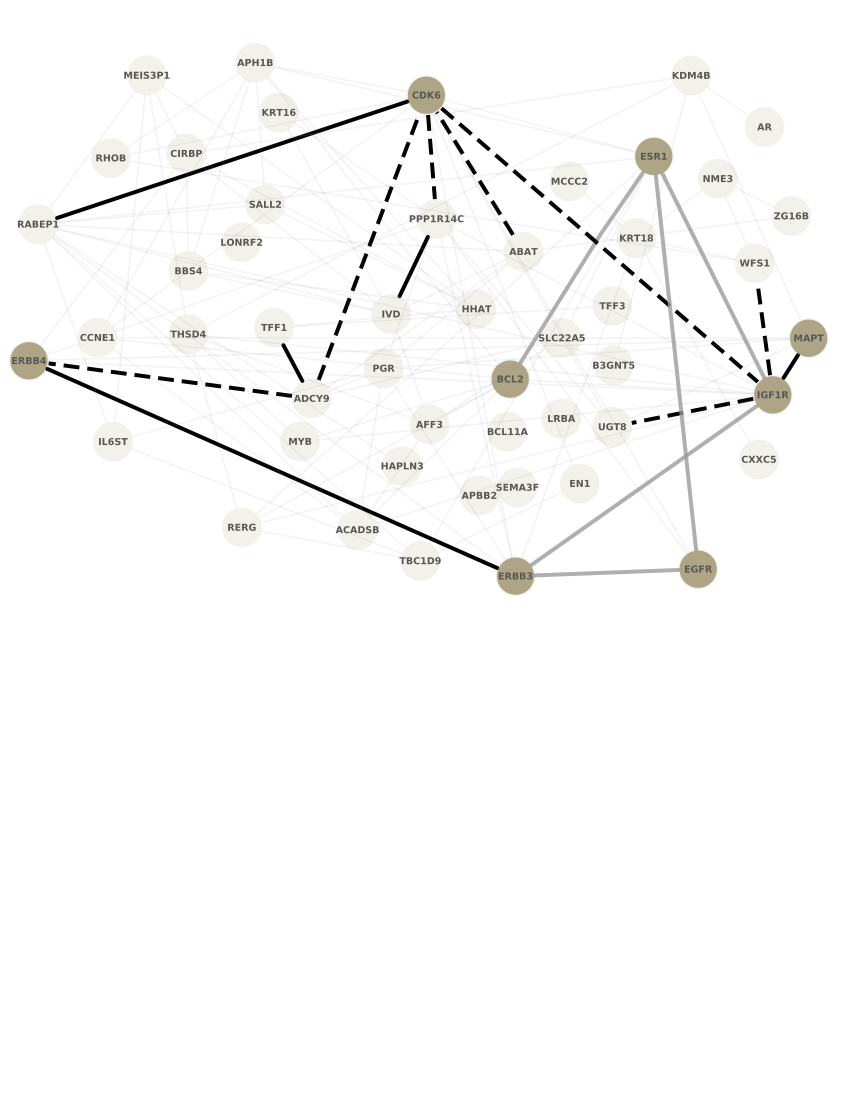
\epsfig{file=\fignet/ERnet.eps, clip=, width=0.5\textwidth}
      \end{tabular}
    \end{tabular}
  \end{overprint}
}

% %==================================================================== 
% \frame{ \frametitle{Playing with penalties: Modularity structure} 
  
%   \paragraph{Prior knowledge on the network topology.} In addition to
%   sparsity, one may assume (\refer{ACM09}) that 
%   \begin{itemize}
%   \item the genes are spread into \emphase{unknown groups} (or
%     'modules')
%   \item regulations between genes are \emphase{driven by group structure}.
%   \end{itemize}
  
%   \bigskip\Pause
%   \paragraph{Inference:} a penalized (variational) E-M algorithm both
%   \begin{itemize}
%   \item infers the (hidden) structure of the groups (see next section),
%   \item fits the precision matrix, using an \emphase{adaptive
%       penalization accounting for the group structure}.
%   \end{itemize}
  
%   \bigskip\Pause
%   \paragraph{SiMoNe package} at 
%   \url{cran.r-project.org/web/packages/simone/}
%   \begin{itemize}
%   \item Graphical group-LASSO,
%   \item Graphical cooperative-LASSO,
%   \item Modular networks.
%   \end{itemize}
% }

%====================================================================
\section{Network Structure}
\frame{ \frametitle{Network Structure} }
%====================================================================

%====================================================================
\subsection{Random graph models}
\frame{ \frametitle{Random graph models} 
%====================================================================
  \paragraph{What for?}
  \begin{itemize}
  \item To be able to better understand networks' structures,
  \item To be able to simulate 'realistic' networks,
  \item To retrieve underlying structures.
  \end{itemize}

  \bigskip\Pause
  \paragraph{Various types of network.} The model must account for the
  network's intrinsic specificities
  \begin{itemize}
  \item Protein-protein interactions: static, binary, undirected,
  \item Gene regulation: static (?), valued, oriented,
  \item Metabolism: bipartite,
  \end{itemize}\Pause 
  and observed characteristics
  \begin{itemize}
  \item sparsity,
  \item heterogeneity,
  \item 'scale-free',
  \item \dots
  \end{itemize}
}

%====================================================================
\frame{ \frametitle{Scale-free model based on bipartite graphs} 

  \paragraph{Topogical specificities.} Many biological network,
  display a (seemingly) 'scale-free' degree distribution, 'small
  world' property and contain a giant component.

  \bigskip\Pause 
  \refer{Bir09b} proved that such characteristics can be derived from
  a simple random graph model, involving a \emphase{hidden layer}.

  \bigskip
  \begin{tabular}{cc}
    \hspace{-.5cm}
    \begin{tabular}{p{.4\textwidth}}
      \onslide+<3->{
        \paragraph{Bipartite graph.} 2 categories of nodes exist,
        with simple between-category connectivity
        rules. \\ 
      }
      \onslide+<4->{
        \smallskip
        \paragraph{Projected graph.} We observe only the projection of
        the complete graph on one category.
        \vspace{3cm}~ 
        }
    \end{tabular}
    & 
    \hspace{-.75cm}
    \begin{tabular}{p{.55\textwidth}}
      \begin{overprint}
        \onslide<3>
        \epsfig{file=\fignet/Bipartite.eps, width=.65\textwidth, clip=} 
        \onslide<4>
        \epsfig{file=\fignet/Bipartite-Proj.eps, width=.65\textwidth, clip=} 
      \end{overprint}
    \end{tabular}
  \end{tabular}
    
  % \begin{tabular}{cc}
  %   \hspace{-.5cm}
  %   \begin{tabular}{p{.6\textwidth}}
  %     \paragraph{Bipartite graphs} depict interactions between \emphase{two
  %       different categories of entities}, e.g. metabolic networks
  %     \begin{itemize}
  %     \item chemical compounds (\emphase{$\bigcirc$}),
  %     \item reactions (or enzymes: \emphase{$\square$}).
  %     \end{itemize}
  %   \end{tabular}
  %   & 
  %   \hspace{-.75cm}
  %   \begin{tabular}{p{.5\textwidth}}
  %     \epsfig{file=\fignet/Bipartite-2.eps, clip=, width=0.4\textwidth}
  %   \end{tabular}
  % \end{tabular}

  % \bigskip\Pause

}

%====================================================================
\frame{ \frametitle{Stochastic block-model for interaction graphs} 

  \paragraph{Heterogeneity.} Many biological networks display
  heterogeneous structures (hubs, highly-connected subsets,
  modularity, \dots) that can not be explained by simple random graph
  models.

  \bigskip\Pause
  \paragraph{Hidden structure.} A standard way to account for such an
  heterogeneity is to assume 
  \begin{itemize}
  \item that each node has some hidden (unknown) characteristics
  \item and that connections between nodes depend on their
    characteristics.
  \end{itemize}

  \bigskip\Pause
  \paragraph{Stochastic Block-Model (SBM)} A simple random graph model:
  \begin{itemize}
  \item Nodes $i = 1\dots n$ are spread into $K$ groups with proportions
    \emphase{$\alpha_1, \dots \alpha_K$},
  \item \emphase{$Z_i$} denotes the \emphase{unobserved label} of node $i$,
  \item \emphase{$X_{ij}$} denotes the presence of an edge between
    nodes $i$ and $j$ 
  \end{itemize}
  $$
  \emphase{\pi_{k\ell}} = \Pr\{X_{ij} = 1 | Z_i=k, Z_j = \ell\}.
  $$
}

%====================================================================
\frame{ \frametitle{Application to a regulatory network}

  \vspace{-.5cm}\hspace{-.75cm}
  \begin{tabular}{ll}
    \begin{tabular}{p{6cm}}
      \paragraph{Regulatory network of {\sl E. coli}:} \\
      directed graph where 
      \begin{itemize}
      \item {Nodes =} operons
      \item {Edges =} regulations:
      \end{itemize}
      $$
      \emphase{\{X_{ij} = 1\}}
      \quad \Leftrightarrow \quad 
      \emphase{i \text{ regulates } j}
      $$

      \onslide+<3->{
        \bigskip
        \paragraph{Meta-graph representation.} \\
        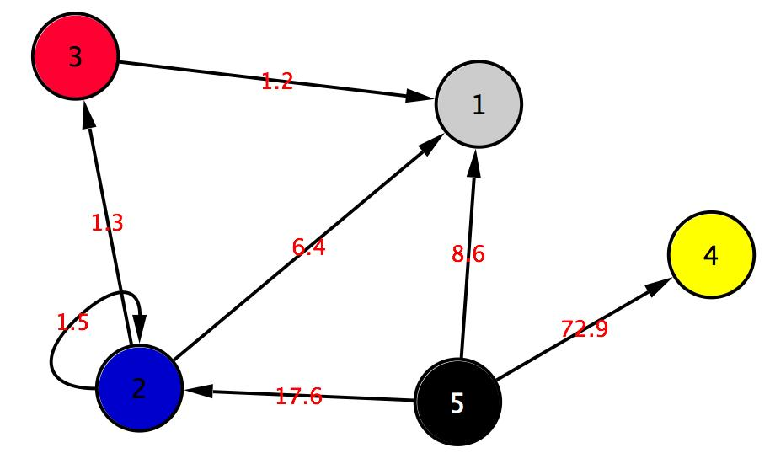
\epsfig{file=\fignet/VEMmetagraphe.ps,
          width=.4\textwidth, clip=}  \\
        \refer{PMD09}

      }
    \end{tabular}
    &
    \begin{tabular}{l}
      \onslide+<2->{
        \hspace{-.75cm}
        \epsfig{file=\fignet/im_EcoliVEM_2.ps,
          width=.45\textwidth, clip=} 
        }
    \end{tabular}
  \end{tabular}
  }

%====================================================================
\subsection{Inference of SBM}
\frame{ \frametitle{Inference of SBM} 
%====================================================================

  \paragraph{Incomplete data model.}
  We observe the edges $\Xbf$, be not the labels $\Zbf$. 
  $$
  \text{\ra We can not deal with the likelihood}
  \qquad
  P(\Xbf) = \sum_{\Zbf} P(\Xbf, \Zbf).
  $$
  
  \Pause
  \paragraph{Classical maximum-likelihood strategy.} E-M algorithms
  alternate
  \begin{enumerate}
  \item[E:] calculation of the conditional distribution of the labels
    \emphase{$P(\Zbf|\Xbf)$},
  \item[M:] parameter estimation with 'known' labels.
  \end{enumerate}\Pause
  In the case of SBM, \emphase{$P(\Zbf|\Xbf)$ is intractable}.
  
  \bigskip \Pause
  \paragraph{Variational E-M.} Replace $P(\Zbf|\Xbf)$ with some
  approximation $Q(\Zbf)$:
  $$
  Q^*(\Zbf) = \arg\min_{Q \in \Qcal} KL\left(Q(\Zbf), P(\Zbf|\Xbf) \right)
  $$
  where $\Qcal$ is a set of \emphase{'friendly' distributions}.
  }

%====================================================================
\frame{ \frametitle{A lot of statistical issues}

  \paragraph{Variational inference.} Including the choice of $K$:
  \begin{itemize}
  \item frequentist version (VEM): \refer{DPR08}
  \item bayesian version (VBEM): \refer{LBA11b}
  \end{itemize}

  \bigskip\Pause
  \paragraph{Understanding variational inference.} As it is an
  approximation we had to
  \begin{itemize}
  \item see if it works: \refer{GDR11}
  \item understand why it works so well: \refer{CDP11}
  \end{itemize}

  \bigskip\Pause
  \paragraph{Alternative inference strategies:} %To scale with large networks
  \begin{itemize}
  \item estimator based on sub-samples of independent edges: \refer{AmM09}
  \item linear estimator based on the degrees: \refer{CDR11}
  \end{itemize}

  \bigskip\Pause
  \paragraph{Generalizations of SBM.} Extend the SBM framework
  \begin{itemize}
  \item to continuous latent space: \refer{DPV10}
  \item to other settings (see next slides)
  \end{itemize}

  % \bigskip\Pause
  % \paragraph{Softwares:}
  % \begin{itemize}
  % \item Stand-alone \emphase{MixNet}:
  %   {\url{stat.genopole.cnrs.fr/software/mixnet/}} 
  % \item R-package \emphase{Mixer}:
  %   {\url{cran.r-project.org/web/packages/mixer/index.html}}
  % \end{itemize}
  }

%====================================================================
\frame{ \frametitle{Generalizations of SBM}

  \onslide+<1->{
    \paragraph{Explicit modeling} allows for generalization. \\
  }
  \begin{tabular}{cc}
    \hspace{-.5cm}
    \begin{tabular}{p{.5\textwidth}}
      \onslide+<2->{
        \paragraph{Overlapping classes:} \\
        Replace 1 drawing per node:
        $$
        Z_i \sim \Mcal(1; \alpha_1, \dots, \alpha_K)
        $$}
      \onslide+<3->{
        with $K$ independent drawings
        $$
        Z_{ik} \sim \Bcal(\alpha_k)
        $$
      \ra \emphase{Overlapping SBM} \\(\refer{LBA11a})}
    \end{tabular}
    & 
    \hspace{-.5cm}
    \begin{tabular}{p{.5\textwidth}}
      \begin{overprint}
        \onslide<2>
        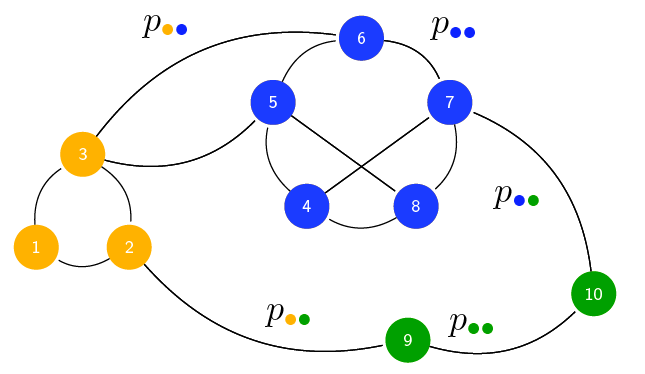
\epsfig{file=\fignet/SBM-CMatias.eps, width=.4\textwidth, clip=} 
        \onslide<3>
        \epsfig{file=\fignet/osbmexample.eps, width=.4\textwidth, clip=} 
      \end{overprint}
    \end{tabular}
  \end{tabular}
  }

%====================================================================
\frame{ \frametitle{Generalizations of SBM}

  \onslide+<1->{
    \paragraph{Explicit modeling} allows for generalization. \\
  }
  \begin{tabular}{cc}
    \hspace{-.5cm}
    \begin{tabular}{p{.5\textwidth}}
      \onslide+<2->{
        \paragraph{Accounting for covariates:} 
        $$
        X_{ij} \sim F(Z_i, Z_j)
        $$
      e.g. $\Esp(X_{ij}) = \lambda_{Z_iZ_j}$ \\}
      \onslide+<3->{
        add covariate $y_{ij}$
        $$
        X_{ij} \sim F(Z_i, Z_j, \emphase{y_{ij}})
        $$
      e.g. $y_{ij} =$ phylogenetic distance, 
      $$
      \Esp(X_{ij}) = \lambda_{Z_iZ_j} \emphase{\beta^{y_{ij}}}.
      $$
      (\refer{MRV10})
    \vspace{1cm}~}
    \end{tabular}
    & 
    \hspace{-.5cm}
    \begin{tabular}{p{.5\textwidth}}
      \onslide+<2->{
        \paragraph{Species interaction network:} \\
        Classification with raw SBM \\
        \vspace{-1cm}
        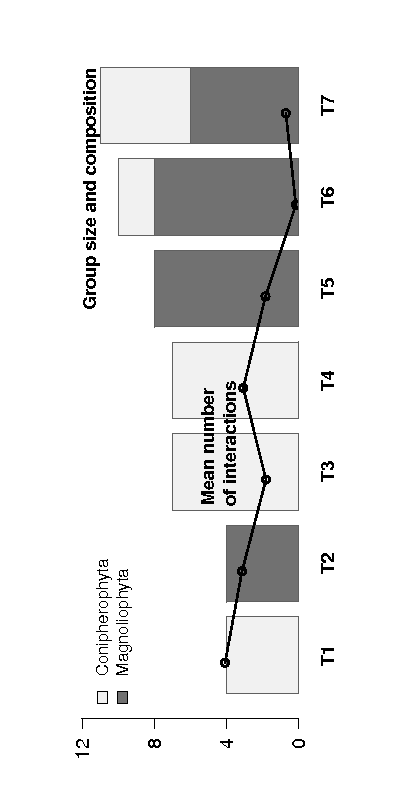
\epsfig{file=\fignet/MRV10_AoAS_Q7_group.eps, width=.4\textheight,
          height=.4\textwidth, clip=, angle=270} \\
        }
      \onslide+<3->{
        \paragraph{Accounting for phylogeny:} \\
        \vspace{-1cm}
        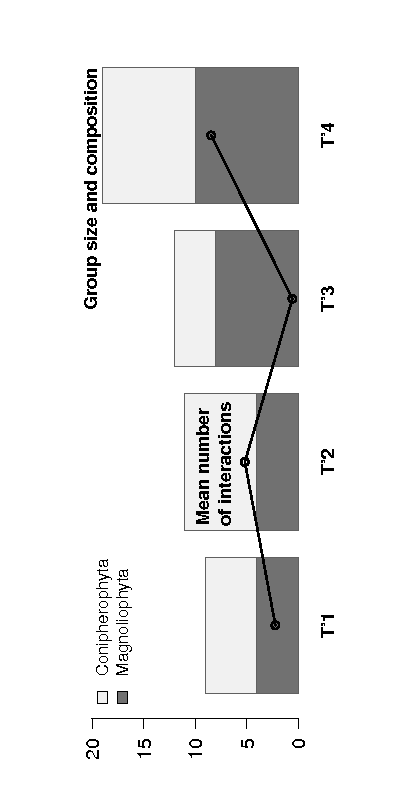
\epsfig{file=\fignet/MRV10_AoAS_Q4_group.eps, width=.4\textheight,
          height=.4\textwidth, clip=, angle=270}
        }
    \end{tabular}
  \end{tabular}
  }

%====================================================================
\section{Network Motifs}
\frame{ \frametitle{Network Motifs} }
%====================================================================

\subsection{Exceptional motifs}
\frame{ \frametitle{Exceptional motifs}

  \paragraph{Motifs = Local patterns} that constitute {functional modules}
  or basic building blocks of complex networks.
  \begin{itemize}
  \item \paragraph{Transcription regulatory networks:} 
    motifs may perform specific regulatory functions
    (e.g. feed-forward loop, bi-fan).
  \item \paragraph{Metabolic motif} may reveal systematic associations of
    reactions in metabolic pathways. 
  \end{itemize}

  \bigskip\Pause
  \paragraph{Motif detection.} To detect 'exceptional motifs', we need
  to
  \begin{enumerate}
  \item Give a precise (topological) definition of a motif $\mbf$;
  \item Be able to count (efficiently) motif occurrences in a given
    network;
  \item Define a random graph model as a null model $G_0$;
  \item Know the (approximate) distribution of the number occurrences
    under the null model $N(\mbf, G_0)$
  \end{enumerate}
  to assess the significance with the $p$-value
  $$
  P\{N(\mbf, G_0) > n_{\text{obs}}\}
  $$

  }

%==================================================================== 
\subsection{Motif definition}
%====================================================================
\frame{\frametitle{Different motifs for different networks}
  \begin{tabular}{cc}
    \hspace{-.5cm}
    \begin{tabular}{p{.45\textwidth}}
      \paragraph{Metabolic networks.} Colored \\graph
      \begin{itemize}
      \item Nodes = reactions
      \item Color = type
      \item Edges = shared compound
      \end{itemize}
    \end{tabular}
    & 
    \hspace{-.5cm}
    \begin{tabular}{p{.45\textwidth}}
      \paragraph{Interaction networks.} (Oriented) graph
      \begin{itemize}
      \item Nodes = proteins, genes
      \item Edges = interactions, regulations
      \end{itemize}
    \end{tabular}
  \end{tabular}

  \Pause
  \begin{tabular}{cc}
    \hspace{-.5cm}
    \begin{tabular}{p{.45\textwidth}}
      \paragraph{Motif.} Connected component with prescribed color
      frequency
      \begin{center}%$$
        \vspace{-.5cm}
        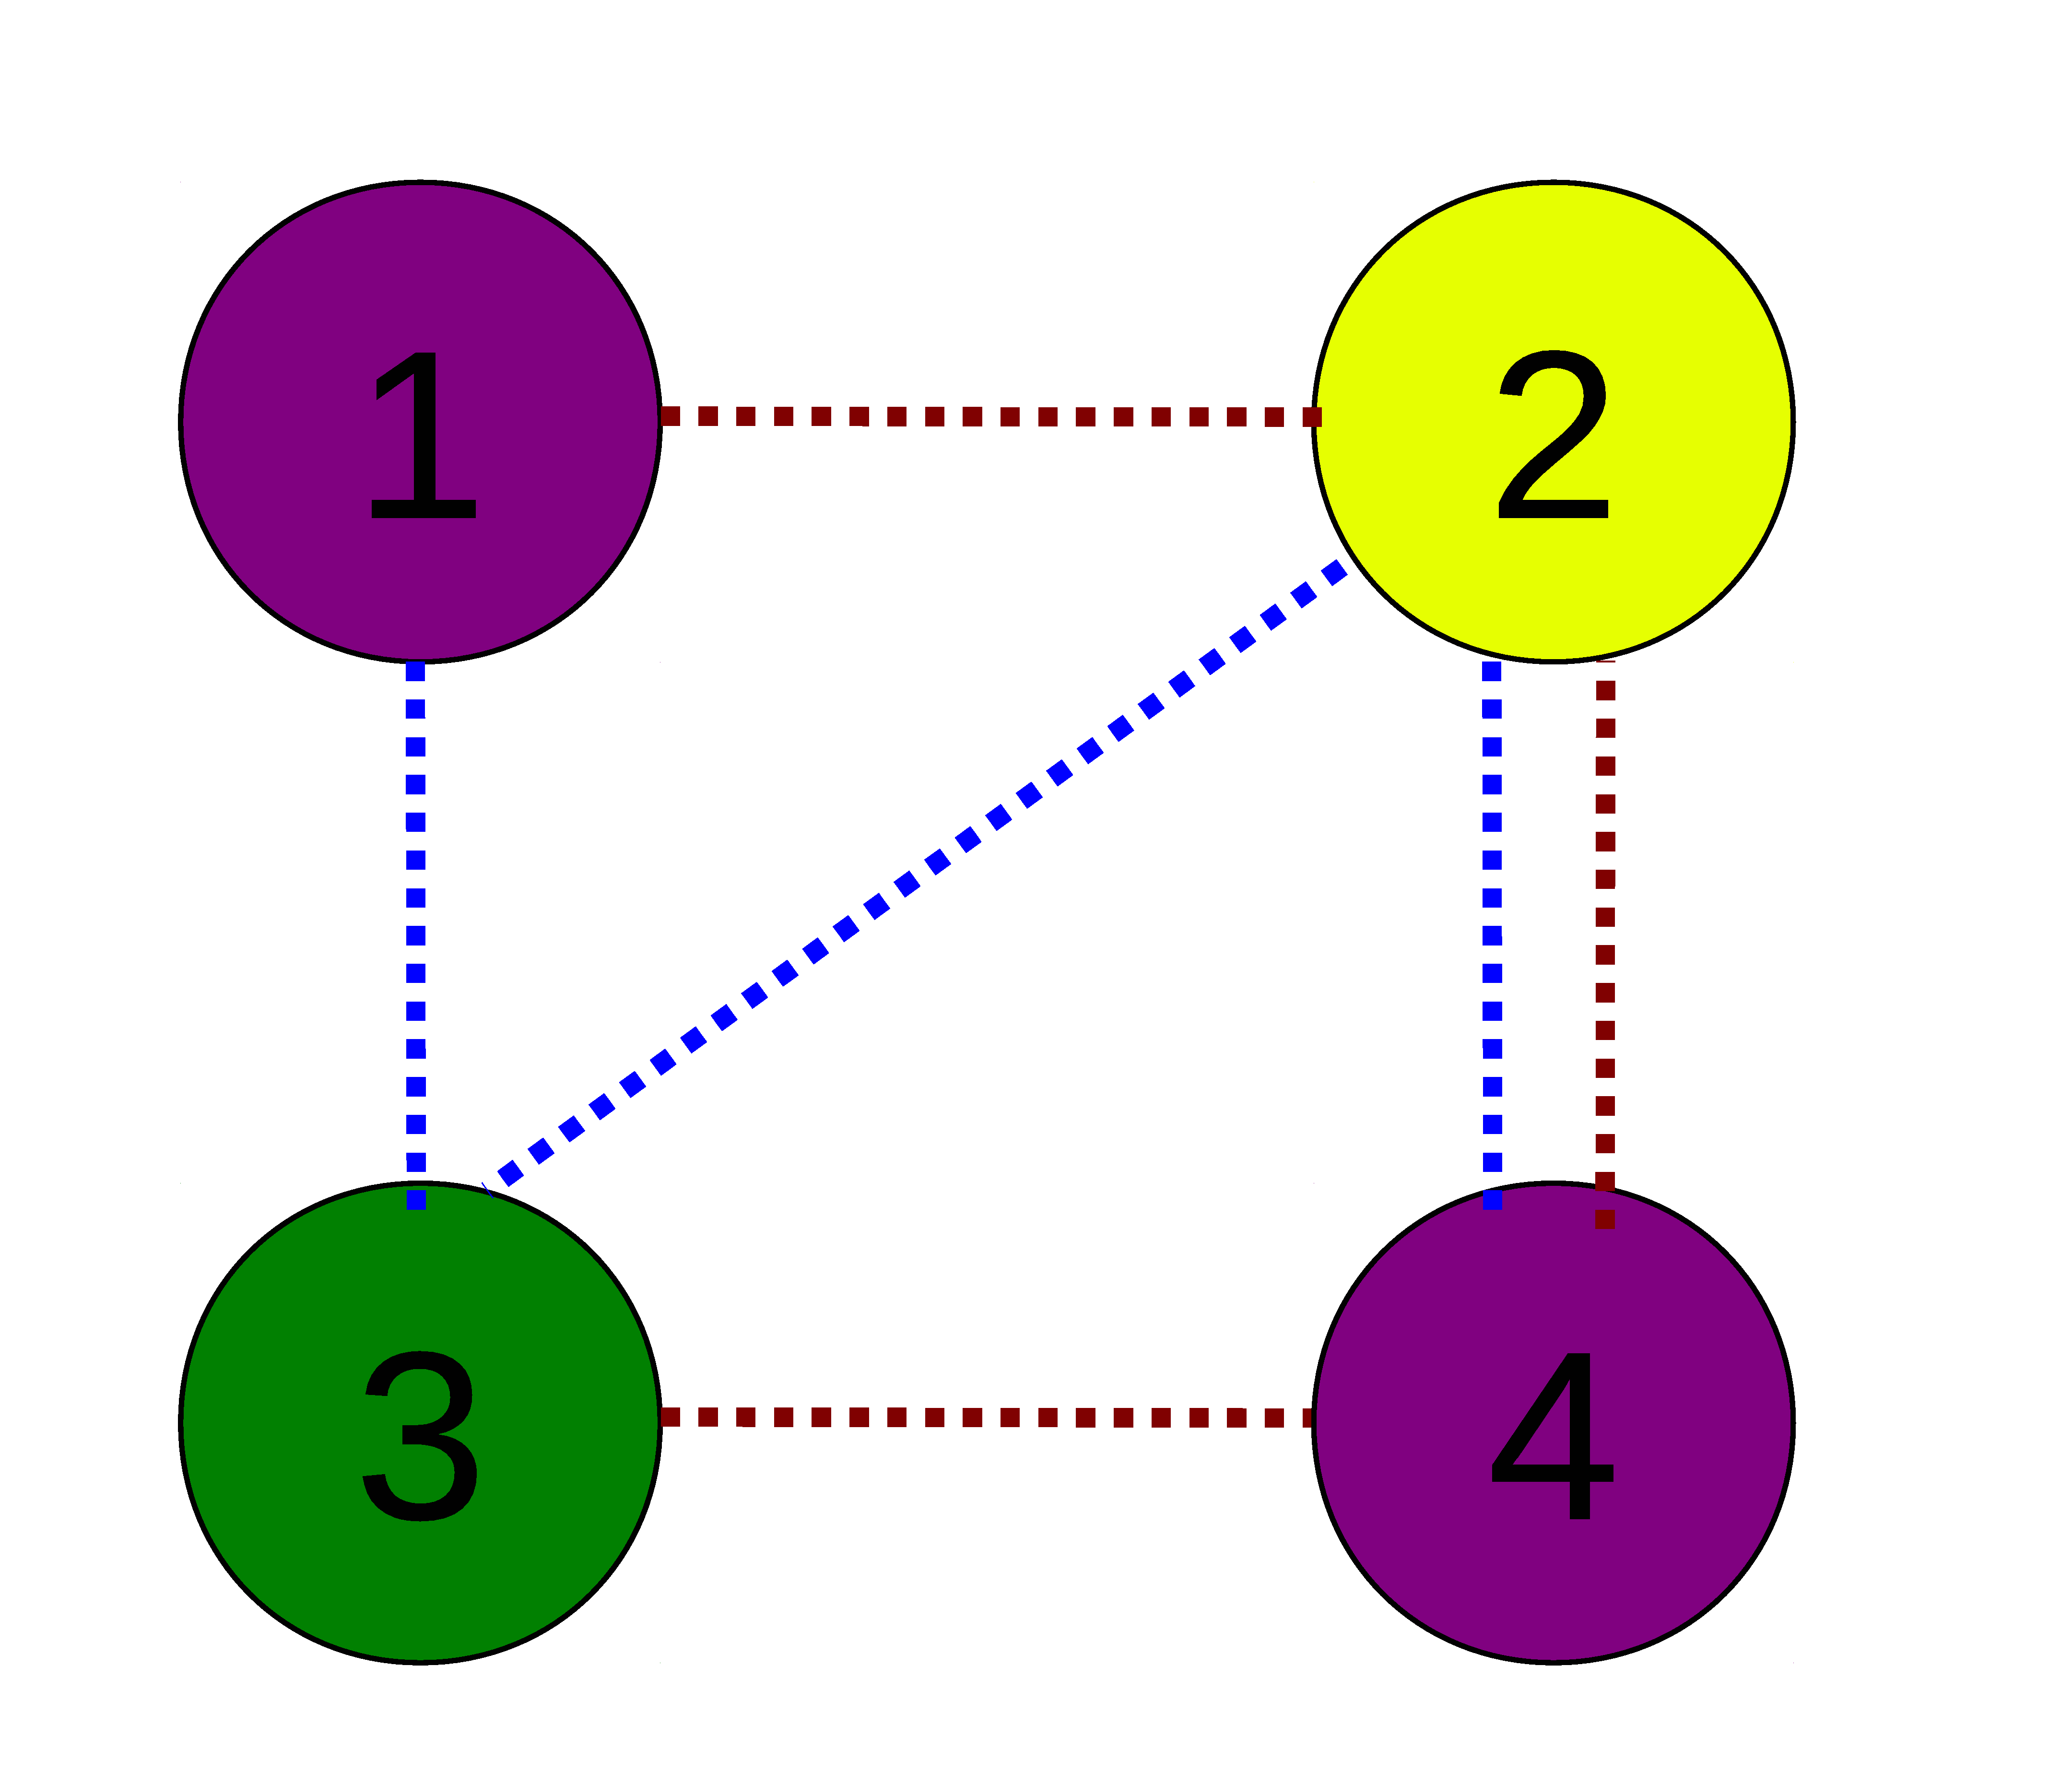
\epsfig{file=\fignet/ColoredMotif-SR.eps, width=.8\textwidth, clip=}
      \end{center}%$$
    \end{tabular}
    & 
    \hspace{-.5cm}
    \begin{tabular}{p{.45\textwidth}}
      \paragraph{Motif.} Connected component with prescribed topology
      \begin{center}%$$
      \epsfig{file=\fignet/version2.eps, width=0.25\textwidth}  
      %\epsfig{file=\fignet/version3.eps, width=0.3\textwidth}  
      %\epsfig{file=\fignet/version1.eps, width=0.3\textwidth} 
      \end{center}%$$
      ~\vspace{4cm}~ 
    \end{tabular}
  \end{tabular}
  }

% %==================================================================== 
% \frame{\frametitle{Coloured motif in metabolic networks}
%   \begin{tabular}{cc}
%     \begin{tabular}{p{0.45\textwidth}}
%       A motif $\mbf$ is defined by a set of $k$ colors (with possible
%       repetitions). \\
%       ~\\
%       \emphase{Colour} = Enzyme classification\\
%       ~\\    
%       A coloured motif $\mbf$ of size $k$ occurs when
%       \begin{itemize}
%       \item a set of $k$ nodes
%       \item composing a \emphase{connected} subgraph
%       \item with \emphase{prescripted} colors
%       \end{itemize}
%       is observed. \\
%     \end{tabular}
%     &
%     \begin{tabular}{p{0.45\textwidth}}
%       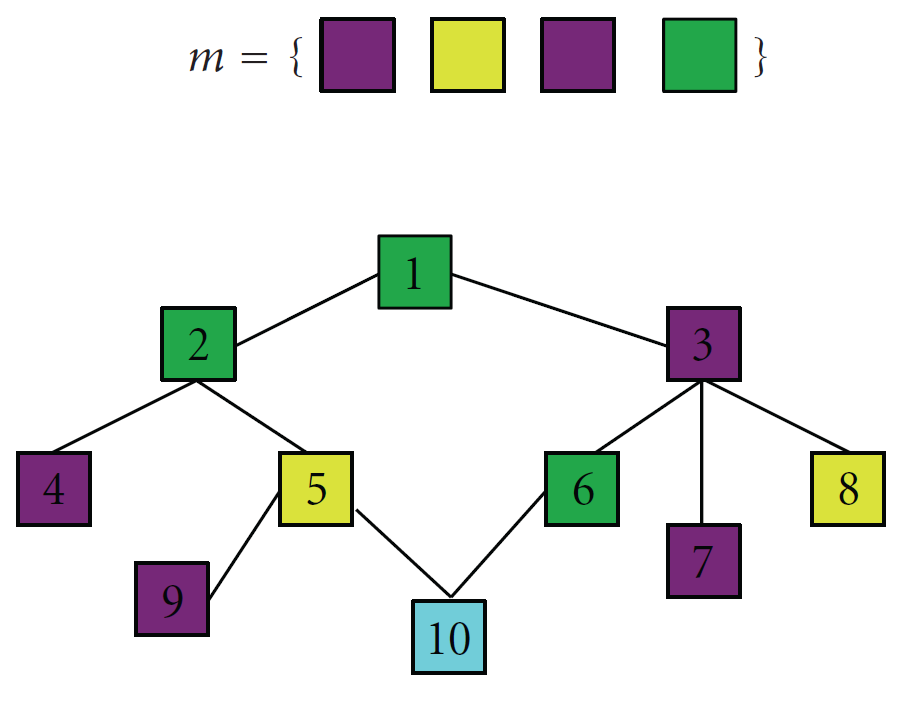
\includegraphics[width=.45\textwidth]{\fignet/SLS09-JBSB-Fig2}
%       \\
%       \\
%       3 occurrences of the motif $m$. \\
%       \\
%       \refer{LFS06}, \refer{SLS09}
%     \end{tabular}
%   \end{tabular}
%   }

% %==================================================================== 
% \frame{\frametitle{Topological motif in interaction networks}

%   \paragraph{Definition.}  A topological motif $\mbf$ is characterized
%   by its ... precise topology, e.g. '$\nabla$', ''$\Vsf$'', ...

%   \bigskip
%   \hspace{-.6cm}
%   \begin{tabular}{cc}
%     \begin{tabular}{p{0.45\textwidth}}
%       \onslide+<2->{
%         \paragraph{Permutations.} For a given motif $\mbf$, we need to
%         consider the set $\Rcal(\mbf)$ of its permutations. \\
%       }
%       \onslide+<3->{
%         \bigskip
%         \paragraph{Occurrences.}
%         A topological motif $m$ of size $k$ occurs when
%         \begin{itemize}
%         \item a set of $k$ nodes
%         \item with \emphase{prescribed} edges
%         \end{itemize}
%         is observed. \\
%         ~\\
%         \emphase{Induced motif}
%         $\neq$ exact occurrence.
%       }
%     \end{tabular}
%     &
%     \begin{tabular}{p{0.45\textwidth}}
%       \onslide+<2->{
%         \vspace{-.5cm}
%         \begin{tabular}{ccc}
%           \epsfig{file=\fignet/version2.eps, width=0.1\textwidth} & 
%           \epsfig{file=\fignet/version3.eps, width=0.1\textwidth} & 
%           \epsfig{file=\fignet/version1.eps, width=0.1\textwidth} 
%           \\
%         \end{tabular}
%         \bigskip
%       }
%       \onslide+<3->{
%         \begin{center}
%         \includegraphics[width=.25\textwidth]{\fignet/PDK08-JCB-Fig1}
%         \end{center}

%         1 occurrence of '$\nabla$'
%         and 5 occurrences '$\Vsf$'. 
%         (\refer{PDK08})
%       }
%     \end{tabular}
%   \end{tabular}
% }

%====================================================================
\subsection{Motif count}
% %====================================================================
% \frame{\frametitle{Motif occurrence}
%   \paragraph{Position.} For a motif of with $k$, we have to consider
%   all ($k$-)position $\alpha$, e.g. all sets of $k$ different nodes
%   taken is ascending order:
%   $$
%   \alpha = (i_1, ... i_k), \qquad i_1 < i_2 < ... < i_k.
%   $$
%   A graph of size $n$ contains \emphase{$\displaystyle{\binom{n}{k}}$
%     positions}. 
  
%   \bigskip\bigskip
%   \paragraph{Motif occurrence:} Binary variable $Y_{\alpha}(\mbf) =
%   \Ibb\{\mbf \text{ occurs at } \alpha\}$ \\ \Pause
%   ~\\
%    \paragraph{Count.} The total number of occurrences is the sum over
%   {all positions} (and {all permutations}) of the binary variables: \\
%   ~\\
%   \begin{tabular}{p{0.4\textwidth}p{0.5\textwidth}}
%     \paragraph{Coloured motif:} 
%     $$
%     N(\mbf) = \sum_{\alpha} Y_{\alpha}(\mbf)
%     $$
%     &
%     \paragraph{Topological motif:} 
%     $$
%     N(\mbf) = \sum_{\alpha} \sum_{\mbf' \in \Rcal(\mbf)} Y_{\alpha}(\mbf')
%     $$
%   \end{tabular}
% }

%==================================================================== 
\frame{\frametitle{Counting occurrences of topological motifs}

%   \paragraph{Coloured motifs.} Already done by \refer{LFS06}.
  \nocite{LFS06}
  
  \paragraph{General principle.} Backtracking along the edges, ranked
  by decreasing degree + pruning.
  
  \bigskip\Pause
  \begin{tabular}{cc}
    \hspace{-.5cm}
    \begin{tabular}{p{.4\textwidth}}
      \paragraph{Pruning.} Given the occurrences of the red, brown and
      green vertices, $n(\mbf)$ is 
      $$
      {5 \choose 2} \times {4\choose 2}
      $$
      without further exploration.
    \end{tabular}
    & 
    \hspace{-.5cm}
    \begin{tabular}{p{.6\textwidth}}
      \epsfig{file=../FIGURES/Graph_08-SR.eps, scale=.2}
    \end{tabular}
  \end{tabular}

  \bigskip\Pause
  From $10^²$ to $10^³$ times faster than FanMod for motif count,
  about $10$ times faster for motif enumeration. (\refer{KGS11})
}
  
%==================================================================== 
\subsection{Null count distribution}
%====================================================================
\frame{\frametitle{Random graph null model}

  \paragraph{The null model} is supposed to generate random
  graphs $G_0$ 'similar' to the observed graphs $G_{\text{obs}}$.

  \bigskip\Pause
  \begin{tabular}{cc}
    \hspace{-.5cm}
    \begin{tabular}{p{.5\textwidth}}
      \paragraph{Metabolic network.}
      \begin{itemize}
      \item Coloured Erdös = Erdös edges + independent colors
      \end{itemize}
    \end{tabular}
    & 
    \hspace{-.5cm}
    \begin{tabular}{p{.5\textwidth}}
      \paragraph{Interaction network.}
      \begin{itemize}
      \item Stochastic block model
      \item Expected degree distribution
      \end{itemize}
    \end{tabular}
  \end{tabular} \\
  \ra Parameters are fitted to the observed graph $G_{\text{obs}}$.

  \bigskip\Pause
  \paragraph{Moments of the count.} For a large class of random graph
  models, \refer{PDK08} propose generic formulas for the first two
  moments:
  $$
  \Esp[N(\mbf, G_0)], \qquad \qquad \Var[N(\mbf, G_0)].
  $$
  The calculation of the variance requires to account for
  \emphase{overlaps between motif occurrences}.  \nocite{MSB06}.
  }

%==================================================================== 
\subsection{(Approximate) distribution}
%====================================================================
\frame{\frametitle{(Approximate) distribution of the count}

  \begin{tabular}{cc}
    \hspace{-.5cm}
    \begin{tabular}{p{.45\textwidth}}
      \paragraph{(Approximate) distribution: } \\
      Polya-Aeppli = geometric Poisson
      $$
      N(\mbf, G_0) \approx \Pcal\Acal(\lambda, a),
      $$
      borrowed from sequences motifs.

      \bigskip\bigskip\Pause
      \paragraph{Parameters} $\lambda$ and $\alpha$ are fitted to the
      first two moments. 

      \bigskip
      \refer{SLS09} \\
      \refer{PDK08}

    \end{tabular}
    & 
    \hspace{-.5cm}
    \begin{tabular}{p{.5\textwidth}}
      \Pause\paragraph{Simulations} for coloured motifs \\~\\
      
      \epsfig{file=\fignet/SLS09-Fig4-BottomLeft.eps,
        width=.5\textwidth} 

      \textcolor{green}{Compound Poisson} provides a better fit than
      \textcolor{red}{Gaussian}. 
    \end{tabular}
  \end{tabular}

  }

% %====================================================================
% \frame{\frametitle{Count distribution under the null model}

%   \paragraph{Null models $G_0$.} See random graph model above:
%   \begin{itemize}
%   \item Coloured motifs: coloured Erdös random graphs (\refer{SLS09})
%   \item Topological motifs: Erdös, SBM + expected degree distribution
%   \end{itemize}

%   \bigskip\Pause
%   \paragraph{Moments of the count.} 
%   \begin{itemize}
%   \item First attempt in \refer{MSB06}.
%   \item \refer{PDK08}: derivation of $\Esp[N(\mbf, G_0)]$ and
%     $\Var[N(\mbf, G_0)]$ for a large class of random graph models.
%   \item Usual difficulty: combinatorial exploration of \emphase{overlaps
%     between occurrences}.
%   \end{itemize}

%   \bigskip\Pause
%   \paragraph{(Approximate) distribution.} Borrowed from sequences
%   motifs:
%   $$
%   N(\mbf, G_0) \approx \text{Compound Poisson}
%   $$
%   }

%====================================================================
\section*{Tools}
\frame{ \frametitle{Tools} 

  \paragraph{Simone.} R package for network inference with graphical
  group-LASSO, graphical cooperative-LASSO, modular networks (\refer{ACM09})
  
  \bigskip\Pause
  \paragraph{MixNet. } Stand-alone software for the stochastic block-model
  \url{stat.genopole.cnrs.fr/software/mixnet/} 
  
  \bigskip
  \paragraph{Mixer. } R package for stochastic block-model (+ some
  extensions)
  
  \bigskip\Pause
  \paragraph{NeMo. } R package for counting and assessing the
  exceptionality of topological motifs in interaction networks
  
  \bigskip
  \paragraph{Paloma. } R package for the detection of locally
  over-represented motif (\refer{Bir09b}).
  % $$
  % \epsfig{file = ../FIGURES/LocalMotif.eps, scale=.5, clip=}
  % $$

  \bigskip
  \paragraph{Motus.} Stand-alone for counting coloured motifs
  (previous to NeMo).
  }

%====================================================================
\section*{In progress / Future Works}
\frame{ \frametitle{In Progress / Future} 

  \paragraph{Metabolic motif.} Motif = pattern satisfying
  stoichiometric properties (\refer{MAB10}, \refer{CMA10},
  \refer{ABC11}) \nocite{ACM12}

  \bigskip\Pause
  \paragraph{Network inference.}
  \begin{itemize}
  \item Network inference for time-course data
  \end{itemize}
    
  \bigskip\Pause
  \paragraph{Network structure.}
  \begin{itemize}
  \item Fitting SBM for large networks
  \item Is there a hidden discrete structure?
  \end{itemize}
    
  \bigskip\Pause
  \paragraph{Network motif.}
  \begin{itemize}
  \item Network distance based on motifs
  \end{itemize}

  }

%====================================================================
\section*{}
\frame{ \frametitle{People} 
  
  \begin{tabular}{p{.3\textwidth}p{.3\textwidth}p{.3\textwidth}}
    \emphase{AgroParisTech/INRA}
    \begin{itemize}
    \item L. Benaroya
    \item A. Channarond
    \item J.-J. Daudin
    \item S. Gazal
    \item M. Koskas
    \item S. Robin
    \end{itemize}
    
    \emphase{INRA-MIG, Jouy}
    \begin{itemize}
    \item S. Schbath
    \end{itemize}
    &
    \emphase{Stat \& Genome, Evry}
    \begin{itemize}
    \item C. Ambroise
    \item E. Birmelé
    \item C. Charbonnier
    \item J. Chiquet
    \item G. Grasseau
    \item M. Jeanmougin
    \item P. Latouche
    \item C. Matias
    \end{itemize}
    &
    \emphase{INRIA~/~LBBE, Lyon}
    \begin{itemize}
    \item V. Acu\~na
    \item V. Cottret
    \item V. Lacroix
    \item V. Miele
    \item P. Milreu
    \item F. Picard
    \item M.-F. Sagot
    \end{itemize}
  \end{tabular}

  \Pause
  \begin{tabular}{cc}
    \hline
    \hspace{-.5cm}
    \begin{tabular}{p{.5\textwidth}}
      \paragraph{SMPGD'12}:  26-27 January, \\
      univ. Lyon - Claude Bernard \\
      \url{smpgd2012.univ-lyon1.fr} \\
    \end{tabular}
    & 
    \hspace{-.5cm}
    \begin{tabular}{p{.5\textwidth}}
      \paragraph{Positions} at AgroParisTech \\
      teaching \& research \\
      in statistics \& genetics/statistics
    \end{tabular}
  \end{tabular} 
}

%====================================================================
{\tiny
  \bibliography{/media/donnees/Biblio/ARC,/media/donnees/Biblio/AST,
    /media/donnees/Biblio/SSB} 
  \bibliographystyle{/media/donnees/LATEX/astats}
  %\bibliographystyle{plain}
  }
%====================================================================

%====================================================================
%====================================================================
\end{document}
%====================================================================
%====================================================================


  \begin{tabular}{cc}
    \hspace{-.5cm}
    \begin{tabular}{p{.5\textwidth}}
    \end{tabular}
    & 
    \hspace{-.5cm}
    \begin{tabular}{p{.5\textwidth}}
    \end{tabular}
  \end{tabular}
